%   Filename    : chapter_4.tex 

\chapter{Results and Discussions}
This chapter presents the results of the machine learning and deep learning analyses conducted on the preprocessed dataset. Preprocessing was performed using Python in Google Colaboratory. The chapter includes the evaluation of various machine learning classifiers, analysis of feature importance, and the application of deep learning models for image-based classification. These approaches aim to identify key predictors and assess classification performance for sex identification in \textit{T. granosa}.

\section{Machine Learning Analysis}
\subsection{Data Exploration}

\begin{figure}[!htbp]
	\centering
	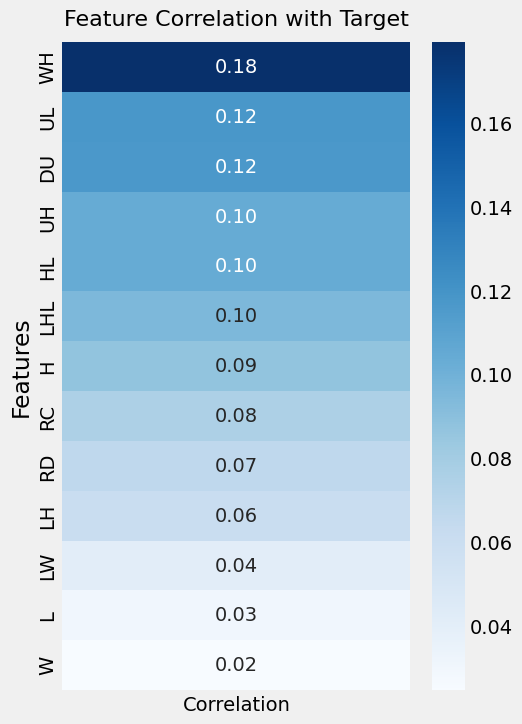
\includegraphics[width=0.4\textwidth]{figures/heatmap.png}
	\caption{Correlation heatmap of morphometric features with the sex of \textit{T. granosa}}
	\label{fig:heatmap}
\end{figure}

Exploratory data analysis was performed to characterize the dataset using visualizations to understand the patterns and correlations within the data. A correlation heatmap was created to assess the relationship between the predictors and the target variable.

The heatmap (see Figure~\ref{fig:heatmap}) revealed three features most correlated with the sex of \textit{T. granosa}: the width-height ratio (r = 0.18), the umbos-length ratio (r = 0.12), and the distance between the umbos (r = 0.12). Each of these features demonstrated a weak positive relationship with the target variable. 

\subsection{Statistical Analysis}

\begin{table}[H]
	\centering
	\small % or \footnotesize or \scriptsize
	\begin{tabular}{lc}
		\hline
		\textbf{Variable} & \textbf{p-value} \\ \hline
		Length & 0.334 \\
		Width & 0.753 \\
		Height & 0.124 \\
		Rib count & 0.251 \\
		Length (Hinge Line) & 0.120 \\
		Distance Umbos & 0.025 \\
		LW\_ratio & 0.011 \\
		LH\_ratio & 0.490 \\
		WH\_ratio & 0.003 \\
		UL\_ratio & 0.019 \\
		HL\_ratio & 0.079 \\
		UH\_ratio & 0.036 \\
		Rib Density & 0.181 \\ \hline
	\end{tabular}
	\caption{Mann-Whitney U Test Results for Sex-Based Feature Comparison}
	\label{tab:mann-whitney}
\end{table}

As part of the exploratory data analysis, statistical testing confirmed that the dataset did not follow a normal distribution. Consequently, the Mann-Whitney U test was applied with a significance level of $\alpha = 0.05$ to compare male and female samples. Out of thirteen features, five showed statistically significant differences. These included: distance between umbos ($p = 0.025$), length-width ratio ($p = 0.011$), umbos-length ratio ($p = 0.019$), width-height ratio ($p = 0.003$), and umbos-height ratio ($p = 0.036$). 

It is important to note that statistical significance does not imply predictive importance. Therefore, further analysis, such as feature importance evaluation, was performed to identify the most informative predictors for classification.

\subsection{Feature Importance Analysis}

\begin{figure}[!htbp]
	\centering
	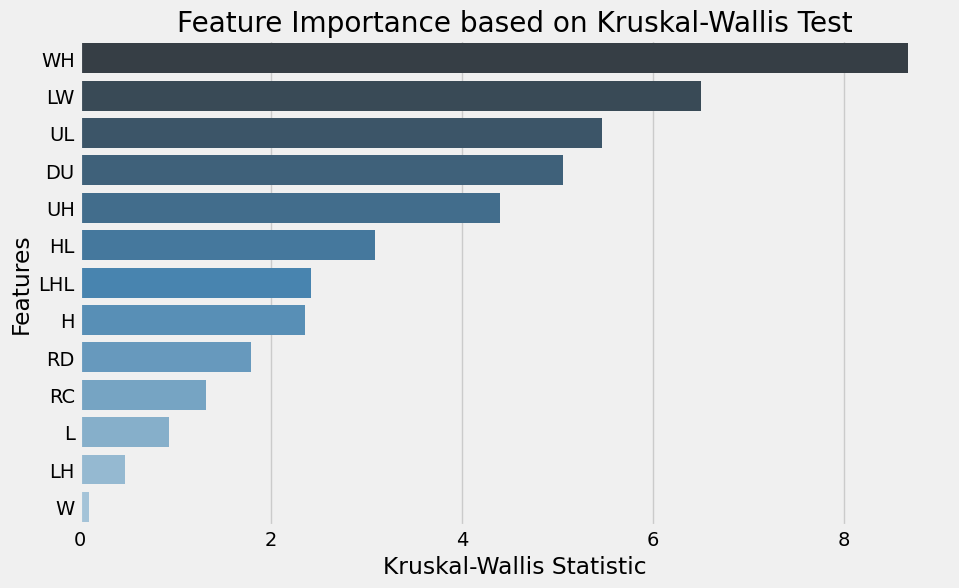
\includegraphics[width=1.0\textwidth]{figures/kw.png}
	\caption{Feature Importance Scores Using the Kruskal-Wallis Test}
	\label{fig:kw}
\end{figure}

Feature importance was assessed using the Kruskal-Wallis test, a non-parametric method that is suitable for evaluating differences in distributions across groups when the data does not follow a normal distribution. This approach was chosen because of the non-normality of the dataset and its robustness in handling continuous and ordinal data without assuming homogeneity of variances. \cite{ribeiro2024}

The analysis showed that the width-to-height ratio (WH\_ratio) had the highest importance score, indicating it is the most statistically significant feature for distinguishing the sex of \textit{T. granosa}. Other notable features included the length-to-width ratio (LW\_ratio), umbos-to-length ratio (UL\_ratio), and the distance between the umbos, all of which contributed significantly to the classification task.

\subsection{Performance Evaluation}
\label{tab:performance-eval}

\begin{table}[H]
	\centering
	\resizebox{\textwidth}{!}{
		\begin{tabular}{lcccccc}
			\hline
			\textbf{Model} & \textbf{Accuracy (\%)} & \textbf{Precision (\%)} & \textbf{Recall (\%)} & \textbf{F1-Score (\%)} \\ \hline
			Support Vector Machine   & 58.62 & 58.62 & 58.62 & 58.44 \\
			Logistic Regression      & 57.83 & 57.83 & 57.83 & 57.61 \\
			K-Nearest Neighbors      & 51.18 & 51.31 & 51.18 & 50.77 \\
			Extra Trees              & 60.24 & 56.98 & 56.69 & 56.39 \\
			Random Forest            & 59.07 & 59.46 & 59.06 & 58.74 \\
			Gradient Boosting        & 60.27 & 60.98 & 60.27 & 59.96 \\
			\cellcolor{celadon}AdaBoost & \cellcolor{celadon}60.63 & \cellcolor{celadon}60.98 & \cellcolor{celadon}60.63 & \cellcolor{celadon}60.39 \\
			\hline
		\end{tabular}
	}
	\caption{Performance Metrics for Models with All 13 Features}
	\label{tab:performance-13-features}
\end{table}

In table~\ref{tab:performance-13-features}, the performance of different machine learning models is presented using the full set of 13 features from the dataset. AdaBoost emerges as the highest-performing model, with an accuracy of 60.63\%, precision of 60.98\%, recall of 60.63\%, and an F1-score of 60.39\%. These results suggest that AdaBoost is particularly effective when utilizing all available features, likely due to its ability to combine multiple weak learners into a more robust model. 

\begin{table}[H]
	\centering
	\resizebox{\textwidth}{!}{
		\begin{tabular}{lcccccc}
			\hline
			\textbf{Model} & \textbf{Accuracy (\%)} & \textbf{Precision (\%)} & \textbf{Recall (\%)} & \textbf{F1-Score (\%)} \\ \hline
			Support Vector Machine   & 63.77 & 64.47 & 63.77 & 63.42 \\
			Logistic Regression      & 63.75 & 63.87 & 63.75 & 63.70 \\
			\cellcolor{celadon}K-Nearest Neighbors      & \cellcolor{celadon}64.16 & \cellcolor{celadon}64.97 & \cellcolor{celadon}64.16 & \cellcolor{celadon}63.75 \\
			Extra Trees              & 62.20 & 59.69 & 59.08 & 58.69 \\
			Random Forest            & 62.96 & 60.10 & 59.85 & 59.54 \\
			Gradient Boosting        & 63.39 & 64.24 & 64.16 & 64.04 \\
			AdaBoost                 & 61.02 & 61.26 & 61.02 & 60.82 \\
			\hline
		\end{tabular}
	}
	\caption{Performance Metrics for Models with 5 Features}
	\label{tab:performance-5-features}
\end{table}

Table~\ref{tab:performance-5-features} presents the performance of the same models using only the top 5 features identified through Kruskal-Wallis feature importance analysis. The top 5 features selected are distance between the umbos, length-to-width ratio, width-to-height ratio, umbos-to-height ratio and umbos-to-length ratio. 

Interestingly, the performance of the models improves with the reduced feature set. K-Nearest Neighbors (KNN) achieves the highest performance in this scenario, with an accuracy of 64.16\%, precision of 64.97\%, recall of 64.16\%, and an F1-score of 63.75\%. These results suggest that KNN benefits from using only the most significant features, showing a notable improvement over its performance when all 13 features are used. 

\section{Deep Learning Analysis}
This section presents the performance of the Convolutional Neural Network (CNN) model in classifying the sex of Tegillarca granosa based on shell morphology. The analysis evaluates the model's ability to distinguish between male and female shell images using various evaluation metrics. This part of the paper includes six subsections: baseline model, comparison of individual and combined angles, training result and hyperparameter tuning, proposed model, learning rates and training behavior per fold, and visualizations.

The machine learning analysis (see Figure~\ref{tab:performance-eval}) revealed that five of the original features produced significant results. The K-Nearest Neighbor (KNN) model achieved an accuracy of 64.16\%, precision of 64.97\%, recall of 64.16\%, and an F1 score of 63.75\%. This section compares the model's performance across different angles based on the results of the machine learning and feature importance analysis.

\subsection{Baseline Model}
This section presents the baseline model with a batch size of 16 and 20 epochs, which will serve as the starting point for comparison and provide a guideline for hyperparameter tuning. The focus will be on one of the angles, specifically the Left Lateral view, since the feature importance analysis using the Kruskal-Wallis Test indicated that the width-to-height ratio had the highest importance score, which is most visible from the Left Lateral view.

\begin{table}[H]
	\centering
	\resizebox{\textwidth}{!}{
		\begin{tabular}{lcccccc}
			\hline
			\textbf{Dataset} & \textbf{Accuracy (\%)} & \textbf{Precision (\%)} & \textbf{Recall (\%)} & \textbf{F1-Score (\%)}  & \textbf{AUC score (\%)}  & \textbf{Loss (\%)} \\ \hline
			Unbalanced   & 65.27 & 71.82 & 58.99 & 63.99 & 73.08 & 0.6122 \\
			\rowcolor{celadon}Balanced     & 67.34 & 69.43 & 64.06 & 65.60 & 74.31 & 0.5981 \\
			\hline
		\end{tabular}
	}
	\caption{Performance Metrics for Unbalanced vs. Balanced Datasets (Batch Size: 16, Epochs: 20)}
	\label{tab:unbalanced-balanced}
\end{table}

The unbalanced dataset, which consisted of 144 male samples and 127 female samples, achieved an accuracy of 65.27\%, precision of 71.82\%, recall of 58.99\%, an F1-score of 63.99\%, an AUC score of 73.08\%, and a loss of 0.6122. However, to address the class imbalance and enhance model performance, random undersampling was performed. This approach resulted in improved performance metrics for the balanced dataset, with an accuracy of 67.34\%, precision of 69.43\%, a recall of 64.06\%, an F1-score of 65.60\%, an AUC score of 74.31\%, and a lower loss of 0.5981.

\section{Comparison of Individual and Combined Angles}
Using the same batch size and number of epochs, performance was compared across all individual angles and the combination of the two highest-performing angles based on accuracy, using a balanced dataset. For the combined analysis, samples from the two selected angles were placed side by side, and a new dataset folder was created for male and female samples. 

\begin{table}[H]
	\centering
	\resizebox{\textwidth}{!}{
		\begin{tabular}{lcccccc}
			\hline
			\textbf{Angle} & \textbf{Accuracy (\%)} & \textbf{Precision (\%)} & \textbf{Recall (\%)} & \textbf{F1-Score (\%)} & \textbf{AUC score (\%)} & \textbf{Loss (\%)} \\ \hline
			Dorsal 	 				& 66.54 & 63.76 & \cellcolor{celadon}77.88 & \cellcolor{celadon}69.96 & 73.09 & 0.6152 \\
			Ventral  				& 67.30 & 69.33 & 66.18 & 66.53 & \cellcolor{celadon}74.87 & 0.6159 \\
			Anterior  				& 51.57 & 31.11 & 6.31  & 10.02 & 65.87 & 0.6825 \\
			Posterior  				& 61.43 & 63.48 & 51.17 & 54.25 & 70.12 & 0.6257 \\
			Left Lateral  			& \cellcolor{celadon}67.34 & \cellcolor{celadon}69.43 & 64.06 & 65.60 & 74.31 & 0.5981 \\
			Right Lateral  			& 65.37 & 67.18 & 59.82 & 62.99 & 71.02 & 0.6115 \\
			Ventral + Left Lateral  & 62.60 & 67.02 & 57.85 & 58.57 & 70.37 & 0.6433 \\
			\hline
		\end{tabular}
	}
	\caption{Performance Metrics for Individual and Combined Angles (Batch Size: 16, Epochs: 20)}
	\label{tab:individual-combined}
\end{table}

Table~\ref{tab:individual-combined} presents the performance metrics for each individual angle and the combination of the two highest-performing angles in terms of accuracy. The Left Lateral view achieved the highest accuracy (67.34\%) and precision (69.43\%), while the Dorsal view obtained the highest recall (77.88\%) and F1-score (69.96\%). Meanwhile, the Ventral view recorded the highest AUC score (74.87\%), indicating its strong ability to distinguish between classes.
Combining the Ventral and Left Lateral views resulted in an overall accuracy of 62.60\%, suggesting that while combined images may provide complementary information, individual angle views still outperformed the combined views under the current experimental setup.

\section{Training Result and Hyperparameter Tuning}
The Left Lateral angle was selected for further optimization. Several experiments were conducted by tuning hyperparameters such as batch size, number of epochs, and activation functions. Each adjustment was compared against the baseline model to enhance performance and develop a robust CNN for sex classification of T. granosa.

The Left Lateral angle was chosen because it achieved the highest accuracy and precision among all individual views, and because the Kruskal-Wallis feature importance analysis indicated that the width-to-height ratio, a feature most visible from the lateral perspective, was the most significant morphological trait for classification. Therefore, focusing on this view was expected to maximize the model's learning capacity and improve classification performance.

\subsection{Batch Size and Number of Epochs}

\begin{table}[H]
	\centering
	\resizebox{\textwidth}{!}{
		\begin{tabular}{lccccccc}
			\hline
			\textbf{Batch Size} & \textbf{No. of Epoch} & \textbf{Accuracy (\%)} & \textbf{Precision (\%)} & \textbf{Recall (\%)} & \textbf{F1-Score (\%)} & \textbf{AUC score (\%)} & \textbf{Loss (\%)} \\ \hline
			16 & 20 & 67.34 & 69.43 & 64.06 & 65.60 & 74.31 & 0.5981 \\
			16 & 30 & 67.73 & 70.17 & 64.06 & 65.72 & 75.76 & 0.5900 \\
			16 & 50 & 67.73 & 70.17 & 64.06 & 65.72 & 75.76 & 0.5900  \\
			32 & 20 & 68.13 & 72.25 & 58.95 & 62.34 & 74.76 & 0.6041 \\
			32 & 30 & 71.28 & 73.17 & 66.89 & 68.27 & 76.76 & 0.5832 \\
			\cellcolor{celadon}32 & \cellcolor{celadon}50 & \cellcolor{celadon}71.68 & \cellcolor{celadon}72.52 & \cellcolor{celadon}69.29 & \cellcolor{celadon}69.12 & \cellcolor{celadon}77.34 & \cellcolor{celadon}0.5824 \\
			64 & 20 & 56.71 & 65.96 & 36.83 & 41.46 & 71.28 & 0.6692 \\
			64 & 30 & 57.95 & 61.94 & 48.12 & 52.66 & 71.22 & 0.6241 \\
			64 & 50 & 61.10 & 62.68 & 56.12 & 56.83 & 73.46 & 0.6086 \\
			\hline
		\end{tabular}
	}
	\caption{Effect of Batch Size and Epoch Values on CNN Model Performance}
	\label{tab:batchsize-epoch}
\end{table}

Table~\ref{tab:batchsize-epoch} shows the results indicating that a batch size of 32 with 50 epochs achieved the best overall performance, with an accuracy of 71.68\%, a precision of 72.52\%, a recall of 69.29\%, an F1-score of 69.12\%, and AUC score of 77.34\%.

In contrast, increasing the batch size to 64 resulted in lower recall and F1-scores, suggesting that smaller batch Sizes (16 or 32) are more effective for this dataset. A moderate batch size of 32 allowed the model to generalize better and maintain stable learning, while too large batch sizes may have led to underfitting.



